\documentclass[11pt]{article}
\usepackage[utf8]{inputenc}

\usepackage[margin=2.1cm]{geometry}
\setlength{\headheight}{14pt}
\usepackage[utf8]{inputenc}
\newcommand{\say}[1]{``#1''}
\usepackage{titling} % multiple title pages

\usepackage{pdfpages}
\usepackage{soul}
\pdfminorversion=7

\usepackage[hidelinks]{hyperref}
\hypersetup{
    colorlinks=false,
    linkcolor=blue,
    filecolor=blue,      
    urlcolor=blue,
}


\title{}
\date{}

\makeatletter
\renewcommand\@bibitem[1]{\item\if@filesw \immediate\write\@auxout
    {\string\bibcite{#1}{Exhibit \the\value{\@listctr}}}\fi\ignorespaces}% <------------
\def\@biblabel#1{Exhibit #1:}% <-------------------
\makeatother


\usepackage{amsmath}
\usepackage{amssymb}
\usepackage[labelfont=bf]{caption}
\usepackage{setspace}\setstretch{1.167} % prerequisite of geometry
\usepackage[utf8]{inputenc}
\usepackage[british, cleanlook]{isodate}
\usepackage[pagewise, modulo, displaymath, mathlines]{lineno}
\usepackage[expansion=false]{microtype}
\usepackage[amssymb]{SIunits}

\usepackage{fancyhdr}
\usepackage{soul}
\usepackage{tikz}
\setlength\parindent{0pt}
\newcommand{\mybullet}{\,\textbullet\,}

\setcounter{tocdepth}{4}
\setcounter{secnumdepth}{4}


\pagestyle{fancy}
\fancyhf{}
\renewcommand{\headrulewidth}{1pt}

\lhead{EB-2 NIW Permanent Residence Petition for Vivek Kumar Mishra}
\cfoot{\thepage}

%% NIW-specific commands
\newcommand{\fie}{Artificial Intelligence, Machine Learning, and Software Engineering}
\newcommand{\dr}{Mr. Vivek Mishra }
\newcommand{\drs}{Mr. Vivek Mishra's }
\newcommand{\qu}[1]{\say{\emph{#1}}}

%% LOR author commands
\newcommand{\pg}{(Corey Graham, Director of Software Engineering, JPMorgan Chase \& Co.)\\}
\newcommand{\ty}{(Dr. Shailesh Chandra, Associate Professor, California State University, Long Beach)\\}
\newcommand{\fb}{(Dr. Maxim A. Dulebenets, Ph.D., P.E., Associate Professor, FAMU-FSU College of Engineering)\\}
\newcommand{\se}{(Dr. Zhenyu Wang, Senior Research Associate, University of South Florida)\\}
\newcommand{\sh}{(Anup Kumar Dubey, Deputy TPO, Anand International College of Engineering)\\}


\begin{document}
\newcommand{\tc}[1]{\textcolor{blue}{#1}}

%% ========================================
%% NIW COVER PAGE AND INITIAL EVIDENCE
%% ========================================

\begin{center}
 \Large{\textbf{Immigrant Petition for Alien Workers}}\\
 \vspace{0.5em}
 \large{\textbf{Employment-Based Second Preference (EB-2)}}\\
 \large{\textbf{National Interest Waiver (NIW)}}\\
 \vspace{0.5em}
 \normalsize{Pursuant to Section 203(b)(2) of the Immigration and Nationality Act}\\
 \normalsize{8 U.S.C. § 1153(b)(2) and 8 C.F.R. § 204.5(k)}
\end{center}

\vspace{4em}


\begin{tabular}{ll}
\textbf{Petitioner and Beneficiary:} & Vivek Kumar Mishra\\
\textbf{Classification Sought:} & Employment-Based Immigration, Second Preference\\
& National Interest Waiver (EB-2 NIW)\\
& Sec. 203(b)(2) INA [8 U.S.C. 1153(b)(2)]\\
\end{tabular}

\vspace{2em}


To whom it may concern,

\vspace{2em}

This letter is respectfully submitted in support of the petition of Mr. Vivek Kumar Mishra for classification as a qualified immigrant under the second preference employment immigration category pursuant to section 203(b)(2) of the Immigration and Nationality Act (``the Act''), with a request for a National Interest Waiver of the job offer and labor certification requirements under section 212(a)(5)(A) of the Act.

This petition demonstrates that \dr meets the requirements for the National Interest Waiver (NIW) as established by the Administrative Appeals Office in \textit{Matter of Dhanasar}, 26 I\&N Dec. 884 (AAO 2016). Specifically, this petition provides evidence that:

\begin{enumerate}
 \item \dr possesses an \underline{advanced degree} (Master of Science in Computer Science from California State University, Long Beach), satisfying the threshold requirement for EB-2 classification under 8 C.F.R. § 204.5(k)(2).
 
 \item \dr satisfies the three-prong test established in \textit{Matter of Dhanasar}:
 \begin{itemize}
  \item \textbf{Prong 1:} \drs proposed endeavor has both \underline{substantial merit} and \underline{national importance}. (Section \ref{sec:prong1})
  \item \textbf{Prong 2:} \dr is \underline{well positioned to advance} the proposed endeavor. (Section \ref{sec:prong2})
  \item \textbf{Prong 3:} On balance, it would be \underline{beneficial to the United States} to waive the requirements of a job offer and labor certification. (Section \ref{sec:prong3})
 \end{itemize}
\end{enumerate}

Pursuant to 8 C.F.R. § 204.5(k), \dr may file an I-140 visa petition for classification under Section 203(b)(2) of the Act as an alien with an advanced degree seeking a National Interest Waiver.

Pursuant to 8 C.F.R. § 204.5(k)(4)(ii), \dr requests that the requirement of a job offer and labor certification be waived because his admission to the United States would be in the national interest.

\pagebreak

%% ========================================
%% INTRODUCTION: THE PROPOSED ENDEAVOR
%% ========================================

\section{The Proposed Endeavor}
\label{sec:endeavor}

\dr proposes to continue advancing the development and deployment of \underline{Artificial Intelligence and Machine Learning systems} for critical national infrastructure in the United States. His proposed endeavor encompasses two interconnected domains:

\begin{enumerate}
    \item \textbf{Enterprise Financial Technology Systems:} Developing AI-integrated platforms serving tens of millions of Americans through systemically important financial institutions, ensuring the security, reliability, and accessibility of the nation's financial infrastructure.
    
    \item \textbf{AI-Driven Intelligent Transportation Systems (ITS) Research:} Applying machine learning methodologies to optimize transportation investment decisions, improve accessibility for underserved communities, and advance sustainable transportation policies aligned with federal infrastructure priorities.
\end{enumerate}

This endeavor directly advances U.S. competitiveness in artificial intelligence---a technology that President Biden's Executive Order 14110 on ``Safe, Secure, and Trustworthy Artificial Intelligence'' (October 30, 2023) identifies as critical to national security and economic prosperity.

\pagebreak

%% ========================================
%% SECTION 1: ADVANCED DEGREE QUALIFICATION
%% ========================================

\section{\dr Possesses an Advanced Degree}
\label{sec:advdegree}

Pursuant to 8 C.F.R. § 204.5(k)(2), \dr qualifies for EB-2 classification based on his possession of an advanced degree.

\textbf{Educational Credentials:}

\begin{itemize}
    \item \textbf{Master of Science in Computer Science} (2021)\\
    California State University, Long Beach\\
    Carnegie Classification: R2 Doctoral University (High Research Activity)\\
    \textit{Evidence: Exhibit AD-1}
    
    \item \textbf{Bachelor of Technology in Information Technology} (2014)\\
    West Bengal University of Technology, India\\
    \textit{Evidence: Exhibit AD-2}
\end{itemize}

\drs Master's degree in Computer Science from California State University, Long Beach satisfies the advanced degree requirement under 8 C.F.R. § 204.5(k)(2), which defines an advanced degree as ``any United States academic or professional degree or a foreign equivalent degree above that of baccalaureate.''

California State University, Long Beach is classified as an R2 Doctoral University under the Carnegie Classification system, indicating ``High Research Activity.'' This classification places CSULB among the top tier of U.S. research universities.

\textbf{Conclusion:} \dr clearly satisfies the advanced degree requirement for EB-2 classification.

\pagebreak

%% ========================================
%% SECTION 2: DHANASAR PRONG 1
%% ========================================

\section{Prong 1: The Proposed Endeavor Has Substantial Merit and National Importance}
\label{sec:prong1}

Under the first prong of the \textit{Dhanasar} framework, \dr must demonstrate that his proposed endeavor has both substantial merit and national importance. This section establishes that \drs work in AI/ML for financial technology and intelligent transportation systems satisfies both elements.

\subsection{Substantial Merit of the Proposed Endeavor}

\drs proposed endeavor has substantial merit based on its technical significance, economic impact, and alignment with critical national priorities.

\subsubsection{Technical Merit: AI/ML Systems at Enterprise Scale}

\dr has demonstrated substantial technical contributions through his work developing AI-integrated systems at JPMorgan Chase \& Co., one of the world's largest financial institutions:

\begin{itemize}
    \item \textbf{Production Impact:} \drs systems process over \underline{5 million customer requests per month} with 99.9\% reliability \cite{metrics}
    \item \textbf{Enterprise Scale:} Platform serves 80+ million Chase cardmembers across the United States \cite{shopsatchase}
    \item \textbf{Technical Leadership:} Designed core backend APIs for ``The Shops at Chase'' e-commerce platform, launched June 2025
\end{itemize}

As Corey Graham, Director of Software Engineering at JPMorgan Chase with 23 years of experience, attests:

\qu{Throughout the development of the Shopping Hub, Vivek played a critical role in building and deploying the core backend services that underpin the platform. He designed APIs that are now part of a mission-critical system, implemented observability and alerting infrastructure to ensure uptime and reliability, and managed secure integrations with external vendors for rewards redemption and settlement.} \cite{corey}

\subsubsection{Technical Merit: Scholarly Research in AI/ML}

Beyond industry contributions, \dr has authored \textbf{8 peer-reviewed scholarly articles} in artificial intelligence, data analytics, and AI-driven intelligent transportation systems (ITS). His research demonstrates substantial technical merit:

\begin{itemize}
    \item \textbf{Federal Funding:} Research funded by U.S. Department of Transportation, Mineta Transportation Institute, and California State University Transportation Consortium
    \item \textbf{Federal Recognition:} Two publications permanently indexed in the National Transportation Library (ROSA P Records dot/61210 and dot/59030)
    \item \textbf{Citations:} 37 citations from researchers worldwide, including cross-citation by Florida DOT-funded research
    \item \textbf{International Impact:} Citations from researchers in the U.S., Italy, Iran, Romania, and other nations
\end{itemize}

Dr. Maxim A. Dulebenets, Ph.D., P.E., Associate Professor at FAMU-FSU College of Engineering, confirms the substantial merit of \drs research:

\qu{Vivek's work has shaped aspects of our freight network modeling and equity-focused analyses in Florida, particularly in how we evaluate accessibility and performance under different policy constraints. In my professional opinion, Vivek's most significant contributions lie in his ability to integrate computer science with advanced technologies such as artificial intelligence, automation, and blockchain to address complex transportation problems.} \cite{maxim}

\subsubsection{Technical Merit: Knowledge Contribution Through Authorship}

\dr has contributed to knowledge dissemination through authorship of ``Design Patterns for AI Agents: A Structured Approach to Building Robust and Intelligent Systems'' (ISBN: 979-8268912371), providing the first structured engineering framework for AI agent architecture. This work has been formally adopted by an accredited academic institution for educational purposes \cite{bookadoption}.

\subsection{National Importance of the Proposed Endeavor}

\drs proposed endeavor has national importance based on its direct relevance to U.S. financial infrastructure stability, federal intelligent transportation systems priorities, and national AI competitiveness.

\subsubsection{National Importance: Critical Financial Infrastructure}

JPMorgan Chase \& Co. is designated as a \textbf{Systemically Important Financial Institution (SIFI)} by the Financial Stability Oversight Council under the Dodd-Frank Wall Street Reform and Consumer Protection Act. This designation signifies that JPMorgan Chase is critical to the stability and functioning of the U.S. financial system:

\begin{itemize}
    \item \textbf{Assets:} Over \$4.1 trillion in assets under custody---the largest financial institution in the United States
    \item \textbf{Customers:} Serves approximately 84 million consumers and 6 million small businesses
    \item \textbf{Designation:} Classified by the U.S. government as systemically important to national financial stability
    \item \textbf{Credit Card Leadership:} Largest credit card issuer in the United States with over 150 million accounts
\end{itemize}

\drs work developing secure, reliable AI-integrated platforms for JPMorgan Chase directly contributes to the stability and security of America's financial infrastructure. Disruption to JPMorgan Chase's systems would have cascading effects throughout the national and global financial systems, underscoring the national importance of reliable platform development.

\subsubsection{National Importance: Federal Transportation Priorities}

\drs AI-driven intelligent transportation systems (ITS) research directly addresses federal priorities, as evidenced by:

\textbf{1. Permanent Indexing in the National Transportation Library}

The National Transportation Library (NTL) is the official repository of the U.S. Department of Transportation, operated by the Bureau of Transportation Statistics. Two of \drs publications are permanently indexed in this federal repository:

\begin{itemize}
    \item \textbf{ROSA P Record dot/61210:} ``Optimizing Multimodal Transportation Access to Support Commuting Among Low-Income Transit Riders with Social Distancing''
    \item \textbf{ROSA P Record dot/59030:} ``Evaluating Innovative Financing Mechanisms for the California High-Speed Rail Project''
\end{itemize}

This federal indexing demonstrates that \drs research has been recognized as a contribution to the national transportation knowledge infrastructure.

\textbf{2. Alignment with Justice40 Initiative}

\drs research on transportation equity for low-income transit riders directly supports the Biden Administration's Justice40 Initiative, which commits 40\% of federal infrastructure investment benefits to disadvantaged communities. His methodology for optimizing multimodal transportation access provides tools for meeting this national priority.

\textbf{3. Adoption by State Department of Transportation}

\drs research methodologies have been adopted in Florida DOT-funded research, demonstrating cross-state implementation:

\qu{Vivek brings an interdisciplinary depth, combining AI, programming, and infrastructure modeling, that is both rare and increasingly essential in modern transportation research. He has anticipated the shift towards data-driven transportation by developing tools that align with academic objectives while remaining deployable for real-world policy evaluation.} \cite{maxim}

\subsubsection{National Importance: AI National Priority Under Executive Order 14110}

On October 30, 2023, President Biden signed Executive Order 14110 on ``Safe, Secure, and Trustworthy Development and Use of Artificial Intelligence,'' declaring AI a national priority. The Executive Order emphasizes:

\begin{itemize}
    \item The need for AI systems that are safe, secure, and trustworthy
    \item The importance of American leadership in AI development
    \item The critical role of AI in economic competitiveness and national security
\end{itemize}

\drs work developing production AI systems, authoring technical frameworks for AI agent design, and conducting peer-reviewed AI research directly advances these national priorities.

\subsection{Conclusion: Prong 1 Satisfied}

\drs proposed endeavor has both substantial merit (enterprise-scale AI systems, peer-reviewed research, technical book authorship) and national importance (SIFI financial infrastructure, federal transportation priorities, AI national competitiveness). The first prong of the \textit{Dhanasar} test is satisfied.

\pagebreak

%% ========================================
%% SECTION 3: DHANASAR PRONG 2
%% ========================================

\section{Prong 2: \dr is Well Positioned to Advance the Proposed Endeavor}
\label{sec:prong2}

Under the second prong of the \textit{Dhanasar} framework, \dr must demonstrate that he is well positioned to advance the proposed endeavor. USCIS evaluates factors including education, skills, knowledge, record of success, model or plan for future activities, and progress toward achieving the endeavor.

\subsection{Education and Knowledge}

\drs educational background provides the foundation for advancing his proposed endeavor in AI/ML:

\begin{itemize}
    \item \textbf{Advanced Degree:} MS in Computer Science from California State University, Long Beach (R2 Doctoral University)
    \item \textbf{Bachelor's Degree:} B.Tech in Information Technology from West Bengal University of Technology
    \item \textbf{Professional Certification:} AWS Certified Cloud Practitioner \cite{aws}
    \item \textbf{IEEE Senior Member:} Member Number 100495418, granted based on demonstration of ``significant performance'' over 5+ years \cite{ieeecert}
\end{itemize}

\subsection{Skills and Expertise}

\dr possesses specialized skills directly relevant to advancing his proposed endeavor:

\begin{itemize}
    \item \textbf{Artificial Intelligence \& Machine Learning:} Published researcher with expertise in AI applications for transportation and financial systems
    \item \textbf{Backend Development:} Expert in API design, system architecture, and distributed systems
    \item \textbf{Cloud Technologies:} AWS certified with production experience in Kubernetes, containerization, and cloud-native development
    \item \textbf{Enterprise Systems:} Experience developing mission-critical systems at Fortune 500 institutions
    \item \textbf{Programming Languages:} Python, Java, SQL, and related data engineering tools
\end{itemize}

\subsection{Record of Success in Advancing Similar Endeavors}

\dr has a documented record of success in advancing the same type of work he proposes to continue:

\subsubsection{Enterprise Financial Technology Success}

At JPMorgan Chase, \dr has successfully:
\begin{itemize}
    \item Designed and deployed core backend APIs for ``The Shops at Chase'' platform (launched June 2025)
    \item Built systems processing 5+ million customer requests monthly with 99.9\% reliability
    \item Implemented observability infrastructure ensuring uptime for mission-critical financial systems
    \item Managed secure integrations with external vendors for rewards settlement and redemption
\end{itemize}

Director Corey Graham attests to this record of success:

\qu{What sets Vivek apart is his ability to approach complex engineering challenges with both precision and foresight. He consistently demonstrated a thoughtful, methodical approach to building scalable services while prioritizing security and operational stability... His work has already been cited in academic research and has directly contributed to the development of nationally deployed platforms at one of the largest banks in the United States.} \cite{corey}

\subsubsection{Transportation Research Success}

\drs academic research record demonstrates successful advancement of transportation optimization:
\begin{itemize}
    \item 8 peer-reviewed publications in AI, data analytics, and intelligent transportation
    \item 37 citations from researchers worldwide
    \item Two publications permanently indexed in the National Transportation Library
    \item Research adopted in Florida DOT-funded studies
    \item Research on California High-Speed Rail financing (\$105 billion infrastructure project)
\end{itemize}

Dr. Zhenyu Wang, Senior Research Associate at the University of South Florida, confirms:

\qu{Vivek Mishra is one of the most promising emerging researchers connecting artificial intelligence with transportation engineering. His work is recognized internationally and has already influenced both academic research and government-funded programs in the U.S. and abroad.} \cite{wang}

\subsubsection{Knowledge Dissemination Success}

\dr has successfully disseminated knowledge through:
\begin{itemize}
    \item Authorship of ``Design Patterns for AI Agents'' (ISBN: 979-8268912371)---adopted by accredited academic institution
    \item Invited ``Eminent Speaker'' at Faculty Development Programme on AI/ML (AICTE-approved institution)
    \item Featured as ``IEEE Impact Creator'' on IEEE Transmitter thought leadership platform
    \item Published speaker profile on IEEE.tv, IEEE's official television network
\end{itemize}

\subsection{Plan for Future Work}

\dr's plan for advancing his proposed endeavor includes:

\begin{enumerate}
    \item \textbf{Continued Enterprise AI Development (1-3 years):} Continue developing AI-integrated financial technology platforms at JPMorgan Chase or similar distinguished institutions, expanding the reach and capabilities of systems serving tens of millions of Americans.
    
    \item \textbf{Applied AI Research (Ongoing):} Continue peer-reviewed research on AI applications for transportation, financial systems, and infrastructure optimization, building on existing collaborations with universities and government agencies.
    
    \item \textbf{Technical Knowledge Contribution (1-5 years):} Expand technical authorship and educational contributions, potentially including additional books, courses, or training materials on AI agent design and enterprise AI implementation.
    
    \item \textbf{Professional Leadership (Ongoing):} Continue peer review service at premier ML conferences (ICLR, NeurIPS) and IEEE committees, contributing to the advancement of AI standards and best practices.
\end{enumerate}

\subsection{Progress Toward Achieving the Endeavor}

\dr has already made substantial progress toward his proposed endeavor:

\begin{itemize}
    \item[$\checkmark$] Currently employed developing AI-integrated platforms at JPMorgan Chase
    \item[$\checkmark$] Systems already serving millions of users with documented reliability metrics
    \item[$\checkmark$] Research already indexed in federal repositories and adopted by state agencies
    \item[$\checkmark$] Technical book already published and adopted by academic institution
    \item[$\checkmark$] Already recognized as thought leader through IEEE platforms and media coverage
\end{itemize}

\subsection{Expert Recognition of \drs Qualifications}

Multiple experts have independently recognized \drs qualifications to advance his proposed endeavor:

\textbf{Dr. Shailesh Chandra, Associate Professor, California State University, Long Beach:}

\qu{These contributions advanced how transportation agencies like Caltrans assess and simulate investment impacts and mobility strategies. His innovations helped bridge traditional transportation models with modern AI tools, improving real-time decision-making and modeling for system resilience, equity, and efficiency.} \cite{chandra}

\textbf{Corey Graham, Director of Software Engineering, JPMorgan Chase:}

\qu{In my view, Vivek represents the qualities of a top-tier engineer: capable, dependable, and able to deliver high-impact results in environments that demand both speed and precision.} \cite{corey}

\subsection{Conclusion: Prong 2 Satisfied}

\drs education (MS Computer Science), skills (AI/ML, cloud, enterprise systems), record of success (JPMorgan production systems, peer-reviewed research, book authorship), plan for future work, and progress toward the endeavor collectively demonstrate that he is well positioned to advance the proposed endeavor. The second prong of the \textit{Dhanasar} test is satisfied.

\pagebreak

%% ========================================
%% SECTION 4: DHANASAR PRONG 3
%% ========================================

\section{Prong 3: On Balance, It Would Be Beneficial to the United States to Waive the Job Offer and Labor Certification Requirements}
\label{sec:prong3}

Under the third prong of the \textit{Dhanasar} framework, USCIS must determine whether, on balance, it would be beneficial to the United States to waive the job offer and labor certification requirements. This involves weighing the benefits of the alien's contributions against the national interest in protecting domestic workers through the labor certification process.

\subsection{The National Interest in \drs Contributions Outweighs Labor Market Protections}

The benefits of \drs continued contributions to U.S. national interests substantially outweigh the protections provided by the labor certification process for several reasons:

\subsubsection{Critical Financial Infrastructure Cannot Wait for Labor Certification}

The labor certification (PERM) process typically takes 12-18 months or longer. Given the critical nature of financial infrastructure and the rapid evolution of AI technology:

\begin{itemize}
    \item JPMorgan Chase is a Systemically Important Financial Institution whose stability affects the entire U.S. financial system
    \item AI systems require continuous development to address emerging security threats and technological changes
    \item Delays in platform development could impact services for 84 million American consumers
    \item The competitive landscape in AI requires rapid deployment of qualified talent
\end{itemize}

\subsubsection{Labor Certification Would Impede Evolving AI Work}

The nature of AI/ML work makes traditional labor certification problematic:

\begin{itemize}
    \item AI development requires flexibility to work across multiple projects and applications
    \item The specific tasks and responsibilities evolve as technology advances
    \item Fixed job descriptions in labor certification do not accommodate the dynamic nature of AI research and development
    \item \drs contributions span both industry (JPMorgan) and academic research---a combination difficult to capture in a single job offer
\end{itemize}

\subsubsection{\drs Unique Combination of Qualifications}

\dr possesses a rare combination of qualifications that makes him difficult to replace through the domestic labor market:

\begin{itemize}
    \item \textbf{Research credentials:} IEEE Senior Member, peer reviewer for top-tier ML conferences (ICLR, NeurIPS)
    \item \textbf{Industry experience:} Production engineer at systemically important financial institution
    \item \textbf{Published author:} Technical book on AI agents adopted by academic institution
    \item \textbf{Federal recognition:} Research indexed in National Transportation Library
\end{itemize}

This combination of academic research credentials with Fortune 500 production experience in AI/ML is uncommon and represents qualifications beyond those typically available in the domestic labor market.

\subsection{The Intrinsic Merit of the Endeavor Supports Waiver}

\textit{Matter of Dhanasar} established that the first two prongs can provide the basis for approval of Prong 3 when the endeavor has such significant potential benefit to the United States that, on balance, a waiver is warranted.

As established in Sections \ref{sec:prong1} and \ref{sec:prong2}:

\begin{itemize}
    \item \drs endeavor supports critical financial infrastructure serving 84 million Americans
    \item His research advances federal transportation priorities and is permanently indexed in government repositories
    \item His work aligns with Executive Order 14110 on AI national priorities
    \item He has demonstrated success in advancing similar endeavors
\end{itemize}

\subsection{Potential Harm from Requiring Labor Certification}

Requiring labor certification would potentially harm U.S. interests by:

\begin{enumerate}
    \item \textbf{Delaying critical infrastructure development:} Platform development at JPMorgan Chase would be delayed by 12-18+ months
    \item \textbf{Limiting flexibility:} Labor certification ties workers to specific job descriptions, reducing ability to adapt to evolving AI needs
    \item \textbf{Risk of losing talent:} Prolonged uncertainty may drive qualified individuals to other countries competing for AI talent
    \item \textbf{Interrupting ongoing work:} \dr is already making contributions that would be interrupted by labor certification requirements
\end{enumerate}

\subsection{No Negative Impact on U.S. Workers}

Waiving the labor certification requirement for \dr would not adversely affect U.S. workers because:

\begin{itemize}
    \item There is documented shortage of AI/ML talent in the United States
    \item \drs specialized qualifications fill a gap rather than displace domestic workers
    \item His contributions (production AI systems, peer-reviewed research, peer review service) benefit the entire field
    \item His knowledge dissemination through books and speaking educates domestic workers
\end{itemize}

\subsection{Conclusion: Prong 3 Satisfied}

On balance, the national interest in \drs continued contributions to financial infrastructure stability, AI-driven intelligent transportation systems research, and AI advancement substantially outweighs the protections afforded by the labor certification process. Requiring labor certification would delay critical work, impede flexible AI development, and potentially harm U.S. competitiveness in artificial intelligence. The third prong of the \textit{Dhanasar} test is satisfied.

\pagebreak

%% ========================================
%% SECTION 5: SUMMARY AND CONCLUSION
%% ========================================

\section{Conclusion: National Interest Waiver Should Be Granted}
\label{sec:conclusion}

This petition has demonstrated that \dr satisfies all requirements for EB-2 classification with a National Interest Waiver:

\subsection{EB-2 Qualification}

\begin{itemize}
    \item[$\checkmark$] \textbf{Advanced Degree:} MS in Computer Science from California State University, Long Beach (R2 Doctoral University)
\end{itemize}

\subsection{Dhanasar Three-Prong Analysis}

\begin{itemize}
    \item[$\checkmark$] \textbf{Prong 1 - Substantial Merit and National Importance:}
    \begin{itemize}
        \item Enterprise AI systems serving 84 million Americans through SIFI financial institution
        \item Research permanently indexed in National Transportation Library
        \item Alignment with Justice40 Initiative and Executive Order 14110 on AI
        \item Technical book providing first structured framework for AI agent architecture
    \end{itemize}
    
    \item[$\checkmark$] \textbf{Prong 2 - Well Positioned to Advance:}
    \begin{itemize}
        \item MS Computer Science from R2 Doctoral University
        \item IEEE Senior Member (top 8\% of 460,000 members)
        \item Current position at JPMorgan Chase developing AI systems
        \item 8 peer-reviewed publications with federal funding and recognition
        \item Record of success with documented production metrics
    \end{itemize}
    
    \item[$\checkmark$] \textbf{Prong 3 - Beneficial to Waive Requirements:}
    \begin{itemize}
        \item Critical financial infrastructure cannot await labor certification
        \item Unique combination of research and industry credentials
        \item Labor certification would impede flexible AI development
        \item No adverse impact on U.S. workers
    \end{itemize}
\end{itemize}

\subsection{Final Determination}

Based on the evidence presented, \dr has demonstrated that:

\begin{enumerate}
    \item He possesses an advanced degree qualifying him for EB-2 classification;
    \item His proposed endeavor in AI/ML for financial technology and transportation infrastructure has substantial merit and national importance;
    \item He is well positioned to advance the proposed endeavor based on his education, skills, record of success, and ongoing progress; and
    \item On balance, it would be beneficial to the United States to waive the job offer and labor certification requirements.
\end{enumerate}

Accordingly, this petition respectfully requests that USCIS approve \drs I-140 petition for EB-2 classification with a National Interest Waiver.

\vspace{2em}

Respectfully submitted,

\vspace{3em}

\rule{6cm}{0.4pt}\\
Vivek Kumar Mishra\\
Self-Petitioner

\pagebreak

%% ========================================
%% BIBLIOGRAPHY - LIST OF EXHIBITS
%% ========================================

\renewcommand\refname{List of Exhibits}

\begin{thebibliography}{99}

\subsection*{Advanced Degree Evidence}

\bibitem{degree}
\textbf{Exhibit AD-1}: Master of Science Degree in Computer Science.\\
Official diploma and transcripts from California State University, Long Beach (2021).

\bibitem{bachelor}
\textbf{Exhibit AD-2}: Bachelor of Technology Degree in Information Technology.\\
Official diploma from West Bengal University of Technology (2014).

\bibitem{eval}
\textbf{Exhibit AD-3}: Credential Evaluation (if applicable).\\
Third-party credential evaluation confirming U.S. equivalency.

\subsection*{Evidence of Substantial Merit and National Importance (Prong 1)}

\bibitem{shopsatchase}
\textbf{Exhibit NI-1}: JPMorgan Chase Press Release - The Shops at Chase Launch.\\
Official press release announcing the launch of The Shops at Chase e-commerce platform in June 2025, serving 80+ million Chase cardmembers.

\bibitem{metrics}
\textbf{Exhibit NI-2}: Chase Shopping Services Production Metrics (Splunk Dashboard).\\
Screenshot from Splunk Enterprise showing production metrics: 5,012,443 user requests, 22,623 orders, and 99.9\% success rate.

\bibitem{rosap1}
\textbf{Exhibit NI-3}: National Transportation Library ROSA P Record dot/61210.\\
Federal repository record for ``Optimizing Multimodal Transportation Access to Support Commuting Among Low-Income Transit Riders.''

\bibitem{rosap2}
\textbf{Exhibit NI-4}: National Transportation Library ROSA P Record dot/59030.\\
Federal repository record for ``Evaluating Innovative Financing Mechanisms for the California High-Speed Rail Project.''

\bibitem{eo14110}
\textbf{Exhibit NI-5}: Executive Order 14110 on Safe, Secure, and Trustworthy AI.\\
White House Executive Order establishing AI as national priority (October 30, 2023).

\bibitem{sifi}
\textbf{Exhibit NI-6}: JPMorgan Chase SIFI Designation Documentation.\\
Evidence of JPMorgan Chase's designation as Systemically Important Financial Institution under Dodd-Frank.

\bibitem{bookadoption}
\textbf{Exhibit NI-7}: Book Adoption Letter from Anand International College of Engineering.\\
Official letter confirming adoption of \drs AI Agents book into permanent library collection.

\bibitem{book}
\textbf{Exhibit NI-8}: Design Patterns for AI Agents - Technical Book.\\
Full text of ``Design Patterns for AI Agents: A Structured Approach to Building Robust and Intelligent Systems'' (ISBN: 979-8268912371).

\subsection*{Evidence of Being Well Positioned to Advance (Prong 2)}

\bibitem{corey}
\textbf{Exhibit WP-1}: Letter of Recommendation from Corey Graham.\\
Detailed letter from Director of Software Engineering at JPMorgan Chase \& Co. (23 years experience) attesting to \drs critical contributions.

\bibitem{maxim}
\textbf{Exhibit WP-2}: Letter of Recommendation from Dr. Maxim A. Dulebenets.\\
Expert testimonial from Associate Professor at FAMU-FSU College of Engineering regarding \drs research impact.

\bibitem{chandra}
\textbf{Exhibit WP-3}: Letter of Recommendation from Dr. Shailesh Chandra.\\
Expert testimonial from Associate Professor at California State University, Long Beach.

\bibitem{wang}
\textbf{Exhibit WP-4}: Letter of Recommendation from Dr. Zhenyu Wang.\\
Expert testimonial from Senior Research Associate at University of South Florida.

\bibitem{ieeecert}
\textbf{Exhibit WP-5}: IEEE Senior Member Certification.\\
Official IEEE Senior Member certificate and membership card (Member Number: 100495418).

\bibitem{aws}
\textbf{Exhibit WP-6}: AWS Certified Cloud Practitioner Certificate.\\
Professional certification demonstrating cloud technology expertise.

\bibitem{rahul}
\textbf{Exhibit WP-7}: Letter of Recommendation from Rahul Vishwakarma.\\
Detailed letter from Research Engineer at WorkOnward (Techstars-backed), holder of 60+ U.S. patents in AI, data processing, and distributed systems.

\bibitem{raoffer}
\textbf{Exhibit WP-8}: Research Assistant Offer Letter from California State University, Long Beach.\\
Official offer letter from Dr. Shailesh Chandra, Assistant Professor at CSULB, documenting research assistantship position (February 2020).

\bibitem{gscholar}
\textbf{Exhibit WP-9}: Google Scholar Citation Profile.\\
Screenshot documenting 37 total citations, H-index of 3, and publication record.

\bibitem{cv}
\textbf{Exhibit WP-10}: Curriculum Vitae.\\
Complete CV documenting education, experience, publications, and achievements.

\subsection*{Scholarly Publications}

\bibitem{pub1}
\textbf{Exhibit SR-1}: Integrating Solar Photovoltaic Systems into the Grid: An Overview of AI Application.\\
Peer-reviewed scholarly article on AI applications for renewable energy.

\bibitem{pub2}
\textbf{Exhibit SR-2}: The Role of Generative AI in Revolutionizing Healthcare, Education, and Finance.\\
Peer-reviewed scholarly article on generative AI applications.

\bibitem{pub3}
\textbf{Exhibit SR-3}: MDPI Sustainability Journal Publication (sustainability-16-08077).\\
Peer-reviewed article published in MDPI Sustainability (Impact Factor: 3.9).

\bibitem{pub4}
\textbf{Exhibit SR-4}: Framework for Rail Transport Inequality Assessment.\\
Most cited publication with 15 citations.

\bibitem{pub5}
\textbf{Exhibit SR-5}: Evaluating Financing Mechanisms and Economic Benefits to Fund Grade Separation Projects.\\
Peer-reviewed publication with 12 citations.

\bibitem{pub6}
\textbf{Exhibit SR-6}: Evaluating Innovative Financing Mechanisms for the California High-Speed Rail Project.\\
Peer-reviewed scholarly article with 7 citations.

\bibitem{pub7}
\textbf{Exhibit SR-7}: Funding the High-Speed Rail: A Case Study of the California Project.\\
Peer-reviewed publication with 3 citations.

\bibitem{pub8}
\textbf{Exhibit SR-8}: Optimizing Multimodal Transportation Access to Support Commuting Among Low-Income Transit Riders.\\
Peer-reviewed article on transportation equity.

\subsection*{Evidence of Expert Recognition}

\bibitem{iclr}
\textbf{Exhibit ER-1}: ICLR 2025 FM-Wild Workshop Reviewer Invitation and Completion.\\
Evidence of peer review service at top-tier ML conference.

\bibitem{neurips}
\textbf{Exhibit ER-2}: NeurIPS 2025 Position Paper Track Reviewer Evidence.\\
Evidence of peer review service at premier ML conference.

\bibitem{ieee_panel}
\textbf{Exhibit ER-3}: IEEE Senior Member Application Review Panel Service.\\
Evidence of service on IEEE membership evaluation panel (June 2025).

\bibitem{ieee_transmitter}
\textbf{Exhibit ER-4}: IEEE Transmitter Impact Creators Profile.\\
Official IEEE thought leadership platform profile.

\bibitem{ieee_tv}
\textbf{Exhibit ER-5}: IEEE.tv Speaker Profile Page.\\
Official speaker profile on IEEE's television network.

\bibitem{fdp}
\textbf{Exhibit ER-6}: Faculty Development Programme Speaker Schedule.\\
Evidence of ``Eminent Speaker'' invitation at AICTE-approved institution.

\end{thebibliography}

\pagebreak

%% ========================================
%% EXHIBIT PAGES
%% ========================================

%% Exhibit macros
\newcommand{\ip}[1]{\includepdf[pages=-]{#1}}
\newcommand{\ex}[2]{
\title{\textbf{\huge{Exhibit #1}}\\
\vspace{3em}
\Large{#2}
}
\author{}
\maketitle
}

%% ========================================
%% ADVANCED DEGREE EXHIBITS
%% ========================================

\ex{AD-1}{Master of Science Degree in Computer Science}
\begin{center}
\textbf{[MS Diploma and Transcripts from CSULB]}\\
California State University, Long Beach (2021)\\
Carnegie Classification: R2 Doctoral University
\end{center}
\newpage

\ex{AD-2}{Bachelor of Technology Degree in Information Technology}
\begin{center}
\textbf{[B.Tech Diploma from WBUT]}\\
West Bengal University of Technology (2014)
\end{center}
\newpage

%% ========================================
%% NATIONAL IMPORTANCE EXHIBITS
%% ========================================

\ex{NI-1}{JPMorgan Chase Press Release - The Shops at Chase Launch}
\ip{criteria/original/evidence/Announcing The Shops at Chase – A New Way for Chase Cardmembers to Shop and Save.pdf}

\ex{NI-2}{Chase Shopping Services Production Metrics (Splunk Dashboard)}
\begin{center}
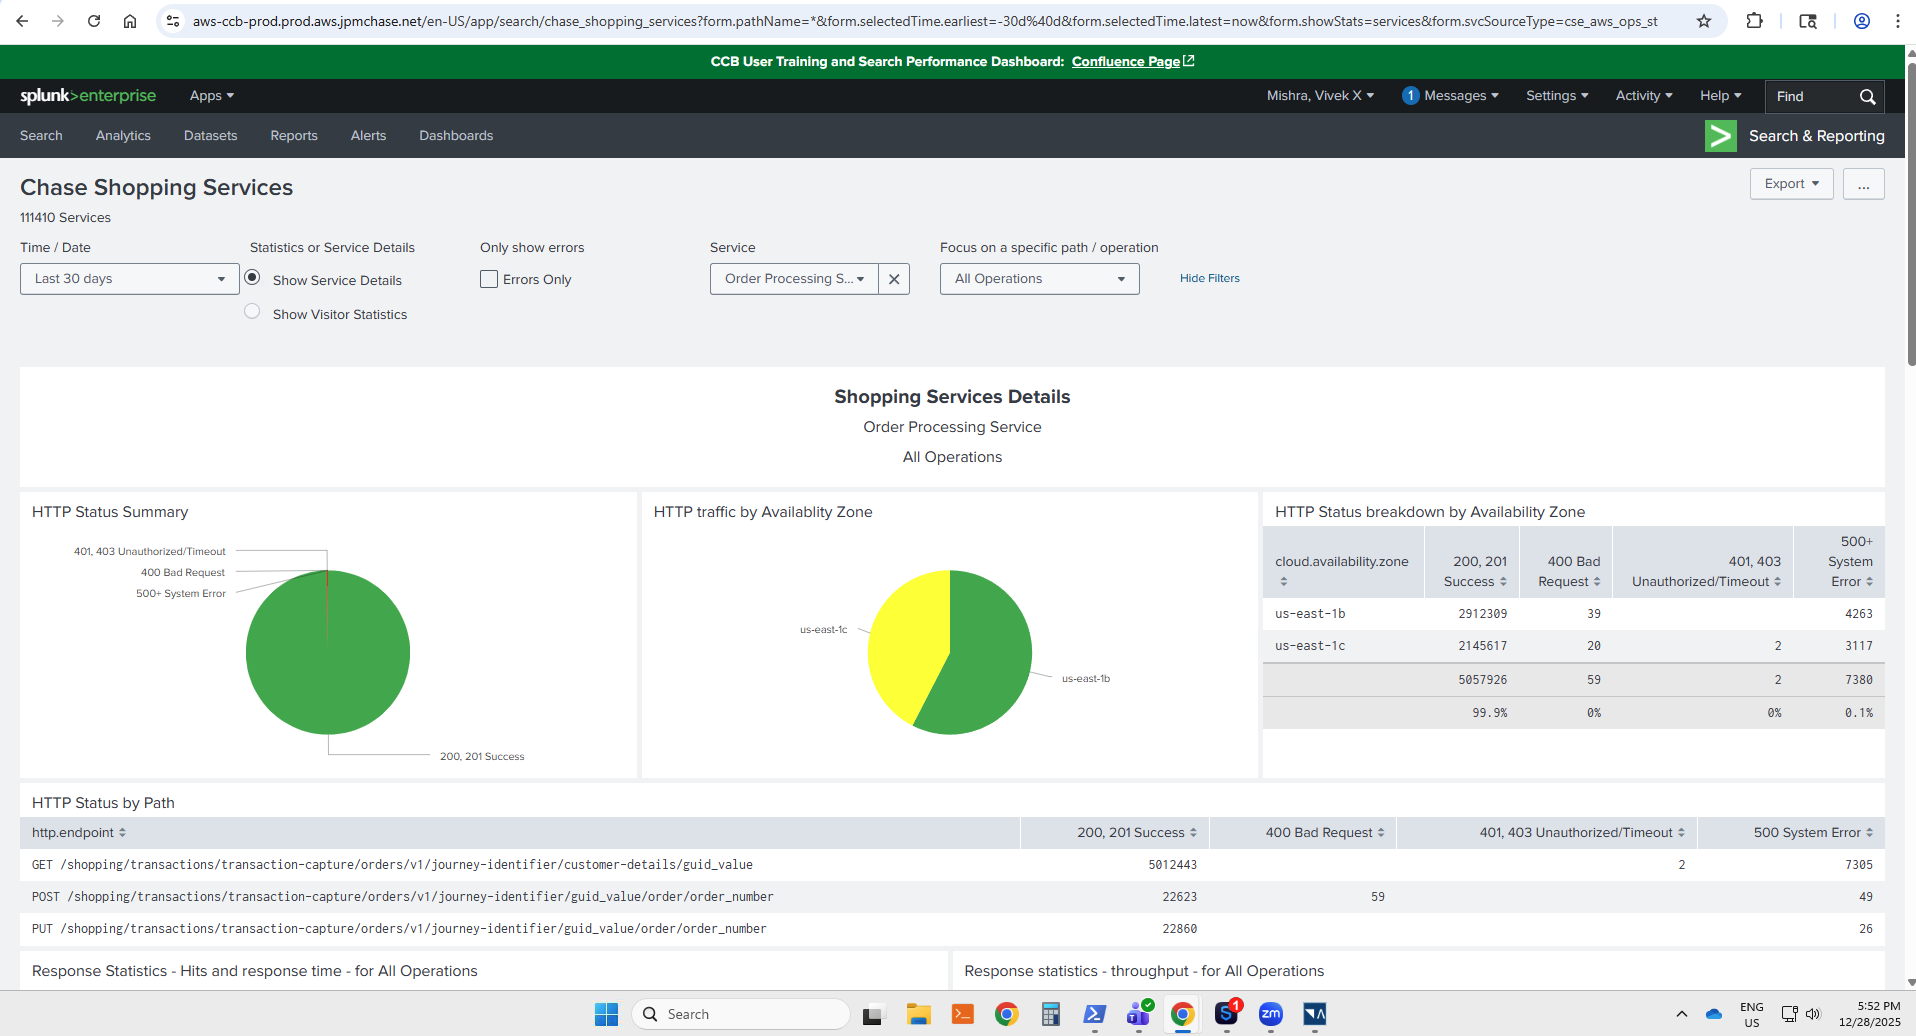
\includegraphics[width=\textwidth]{criteria/original/evidence/chaseWork.png}
\end{center}
\newpage

\ex{NI-3}{National Transportation Library ROSA P Record dot/61210}
\begin{center}
\textbf{[Print from rosap.ntl.bts.gov/view/dot/61210]}\\
\vspace{1em}
Federal repository record for:\\
``Optimizing Multimodal Transportation Access to Support Commuting\\
Among Low-Income Transit Riders with Social Distancing''\\
\vspace{1em}
Report Number: 22-11\\
DOI: 10.31979/mti.2022.2140
\end{center}
\newpage

\ex{NI-4}{National Transportation Library ROSA P Record dot/59030}
\begin{center}
\textbf{[Print from rosap.ntl.bts.gov/view/dot/59030]}\\
\vspace{1em}
Federal repository record for:\\
``Evaluating Innovative Financing Mechanisms for the California High-Speed Rail Project''\\
\vspace{1em}
Report Number: 21-06, CA-MTI-2047\\
DOI: 10.31979/mti.2021.2047
\end{center}
\newpage

\ex{NI-5}{Executive Order 14110 on Safe, Secure, and Trustworthy AI}
\begin{center}
\textbf{[Print from whitehouse.gov]}\\
\vspace{1em}
Executive Order on the Safe, Secure, and Trustworthy\\
Development and Use of Artificial Intelligence\\
\vspace{1em}
October 30, 2023
\end{center}
\newpage

\ex{NI-6}{JPMorgan Chase SIFI Designation Documentation}
\begin{center}
\textbf{[FSOC Documentation of Systemically Important Financial Institution Designation]}\\
\vspace{1em}
JPMorgan Chase \& Co.\\
Total Assets: \$4.1+ Trillion\\
Customers: 84 Million Consumers\\
Designation: Systemically Important Financial Institution (SIFI)
\end{center}
\newpage

\ex{NI-7}{Book Adoption Letter from Anand International College of Engineering}
\ip{criteria/original/evidence/Appreciation Letter_Mr. Vivek Kumar Mishra.pdf}

\ex{NI-8}{Design Patterns for AI Agents - Technical Book}
\ip{criteria/original/evidence/AgentSystemDesign_vivek_IEEE.pdf}

%% ========================================
%% WELL POSITIONED EXHIBITS
%% ========================================

\ex{WP-1}{Letter of Recommendation from Corey Graham, Director of Software Engineering}
\ip{LOR/FinalLetters/LoR - Corey Graham_FINAL.pdf}

\ex{WP-2}{Letter of Recommendation from Dr. Maxim A. Dulebenets}
\ip{criteria/scholar/LOR/MaximLetter.pdf}

\ex{WP-3}{Letter of Recommendation from Dr. Shailesh Chandra}
\ip{LOR/FinalLetters/DrChandra.pdf}

\ex{WP-4}{Letter of Recommendation from Dr. Zhenyu Wang}
\ip{LOR/FinalLetters/DrWang.pdf}

\ex{WP-5}{IEEE Senior Member Certification}
\ip{criteria/member/evidence/IEEE/MEMIEEE500.pdf}

\ex{WP-6}{AWS Certified Cloud Practitioner Certificate}
\ip{criteria/critical/evidence/AWS Certified Cloud Practitioner certificate.pdf}

\ex{WP-7}{Letter of Recommendation from Rahul Vishwakarma, Research Engineer}
\ip{LOR/FinalLetters/Rahul_Vishwakarma.pdf}

\ex{WP-8}{Research Assistant Offer Letter from California State University, Long Beach}
\begin{center}
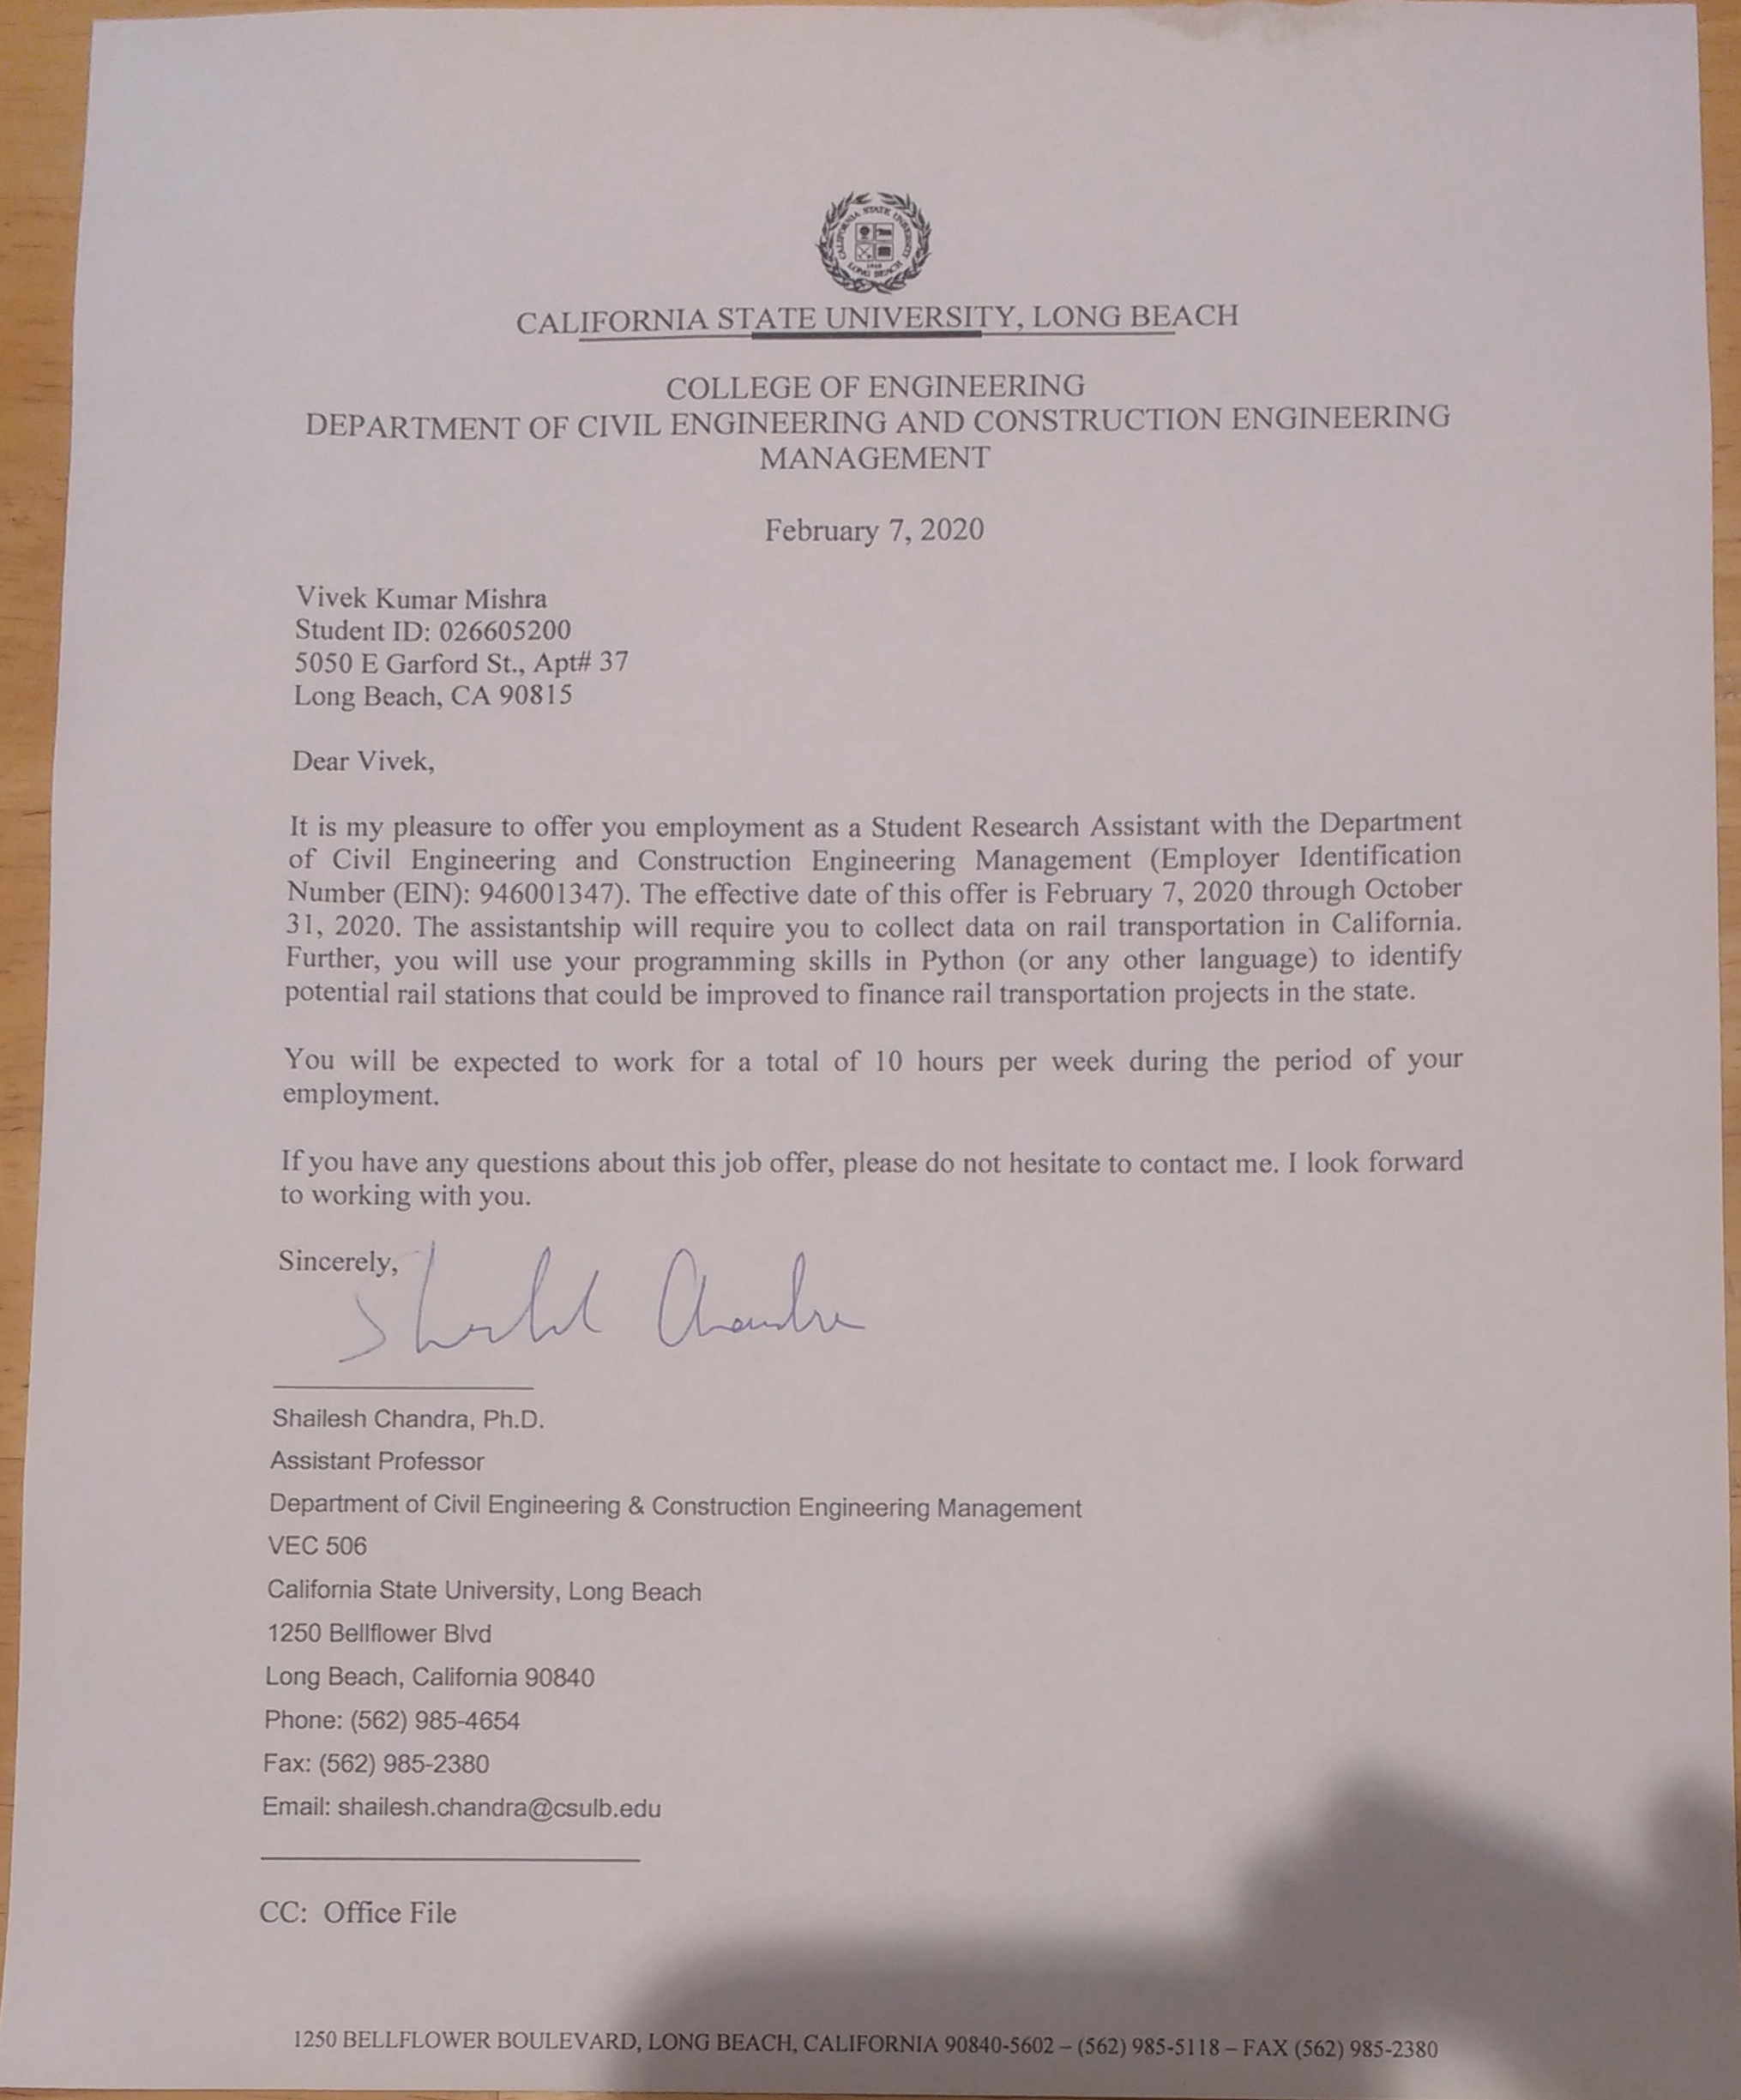
\includegraphics[width=0.8\textwidth]{criteria/critical/evidence/RA_OFFER_Letter.jpg}
\end{center}
\newpage

\ex{WP-9}{Google Scholar Citation Profile}
\begin{center}
\textbf{[Print from Google Scholar]}\\
\url{https://scholar.google.com}\\
\vspace{1em}
37 Total Citations, H-Index: 3
\end{center}
\newpage

\ex{WP-10}{Curriculum Vitae}
\begin{center}
\textbf{[Complete CV]}\\
Documenting education, experience, publications, and achievements
\end{center}



%% ========================================
%% SCHOLARLY PUBLICATION EXHIBITS
%% ========================================

\ex{SR-1}{Integrating Solar Photovoltaic Systems into the Grid}
\ip{criteria/scholar/evidence/Integrating-Solar-Photovoltaic-Systems-into-the-Grid-An-Overview-of-AI-Application.pdf}

\ex{SR-2}{The Role of Generative AI}
\ip{criteria/scholar/evidence/The Role of Generative AI.pdf}

\ex{SR-3}{MDPI Sustainability Journal Publication}
\ip{criteria/scholar/evidence/sustainability-16-08077.pdf}

\ex{SR-4}{Framework for Rail Transport Inequality Assessment}
\ip{criteria/scholar/evidence/Connectivity evaluations.pdf}

\ex{SR-5}{Evaluating Financing Mechanisms and Economic Benefits}
\ip{criteria/scholar/evidence/Evaluating Financing Mechanisms and Economic Benefits to Fund Gra.pdf}

\ex{SR-6}{Evaluating Innovative Financing Mechanisms}
\ip{criteria/scholar/evidence/Evaluating Innovative Financing.pdf}

\ex{SR-7}{Funding the High-Speed Rail}
\ip{criteria/scholar/evidence/FundingHighSpeed.pdf}

\ex{SR-8}{Optimizing Multimodal Transportation Access}
\ip{criteria/scholar/evidence/Optimizing Multimodal Transportation Access to Support Commuting.pdf}

%% ========================================
%% EXPERT RECOGNITION EXHIBITS
%% ========================================

\ex{ER-1}{ICLR 2025 FM-Wild Workshop Reviewer Evidence}
\ip{criteria/judge/evidence/OpenReview/ICLR_2025_FM-Wild_Reviewer_Invitation.pdf}
\ip{criteria/judge/evidence/OpenReview/ICLR_2025_FM-Wild_Paper62_Review_Posted.pdf}

\ex{ER-2}{NeurIPS 2025 Position Paper Track Reviewer Evidence}
\ip{criteria/judge/evidence/OpenReview/NeurIPS_2025_Position_Paper_Reviewer_Invitation.pdf}

\ex{ER-3}{IEEE Senior Member Application Review Panel Service}
\ip{criteria/judge/evidence/IEEE Review/Invitation to the Senior Member Application Virtual Review Panel - June 2025.pdf}
\ip{criteria/judge/evidence/IEEE Review/Thank you letter template-SM Panelist_100495418.pdf}

\ex{ER-4}{IEEE Transmitter Impact Creators Profile}
\begin{center}
\textbf{[Print from IEEE Transmitter]}\\
\url{https://transmitter.ieee.org/author/vivekmishra/}
\end{center}
\newpage

\ex{ER-5}{IEEE.tv Speaker Profile Page}
\begin{center}
\textbf{[Print from IEEE.tv]}\\
\url{https://ieeetv.ieee.org/speaker/vivek-mishra}
\end{center}
\newpage

\ex{ER-6}{Faculty Development Programme Speaker Schedule}
\ip{criteria/original/evidence/FDP_Program.pdf}

\end{document}
